%----------------------------------------------------------------------------------------
%	PACKAGES AND OTHER DOCUMENT CONFIGURATIONS
%----------------------------------------------------------------------------------------

\documentclass[10pt, a4paper, oneside]{article} % Paper size, default font size and one-sided paper

\usepackage{nomencl}
\usepackage{hyperref}
\usepackage{setspace}
\usepackage{fancyhdr}
\usepackage[utf8]{inputenc}
\usepackage{graphicx}
\usepackage{color}
\usepackage{epstopdf}
\usepackage[final]{pdfpages}
\usepackage[utf8]{inputenc}
\usepackage{float}

\usepackage[margin=1in]{geometry}
\usepackage[square, numbers, comma, sort&compress]{natbib} 
%\makenomenclature
\renewcommand{\nomname}{Time Zones}
\newcommand{\solidareit}{\textsc{s}olidare-\textsc{it} }
\title{\ttitle} % Defines the thesis title - don't touch this

\begin{document}
%\frontmatter % Use roman page numbering style (i, ii, iii, iv...) for the pre-content pages

\setstretch{1.2} % Line spacing of 1.3

% Define the page headers using the FancyHdr package and set up for one-sided printing
\fancyhead{} % Clears all page headers and footers
\rhead{\thepage} % Sets the right side header to show the page number
\lhead{} % Clears the left side page header

\pagestyle{fancy} % Finally, use the "fancy" page style to implement the FancyHdr headers

\newcommand{\HRule}{\rule{\linewidth}{0.5mm}} % New command to make the lines in the title page

%----------------------------------------------------------------------------------------
%	TITLE PAGE
%----------------------------------------------------------------------------------------


\definecolor{darkblue}{rgb}{0.1,0.3,0.7}
\definecolor{red}{rgb}{1.0,0.2,0.2}
\definecolor{darkgreen}{rgb}{0.2,0.5,0.2}


\begin{titlepage}

\begin{tabular}{cc}

\begin{minipage}{0.49\textwidth}
\begin{flushleft}

\includegraphics[scale=0.1]{./Figures/logoingisbleu.jpg} % University/department logo - uncomment to place it
\end{flushleft}
\end{minipage}

&
 \begin{minipage}{0.42\textwidth}
\begin{flushright}

\includegraphics[scale=0.5]{./Figures/epl.jpg} % University/department logo - uncomment to place it
\end{flushright}
\end{minipage}
\end{tabular} 



\begin{center}
\vspace{13em}
\textsc{\LARGE lingi2263 : Computational Linguistics }\\[2cm] % University name

 \vspace{1em}
\HRule \\[0.5cm] % Horizontal line
{\huge  Group 2 : Project 3}\\[0.35cm] % Thesis title
\HRule \\[1.5cm] % Horizontal line
 

\begin{tabular}{ccc}
\begin{minipage}{0.55\textwidth}
\begin{flushleft} \large
\emph{Authors:}\\{
Crochelet Martin (2236-10-00)\\
Baugnies Benjamin (6020-10-00)}
\end{flushleft}
\end{minipage} & \begin{minipage}{0.41\textwidth}
\centering
\begin{flushright} \large
\emph{Professor:}\\{
Pierre Dupont\\
Cédric Fairon\\
}
\end{flushright}
\end{minipage}\\[3cm] \\ 
\end{tabular} 

\vspace{4em}


 \begin{center}
{\large 2013 - 2014}\\[4cm] % Date 
 \end{center}


\vfill
\end{center}

\end{titlepage}

%----------------------------------------------------------------------------------------
%	LIST OF CONTENTS/FIGURES/TABLES PAGES
%----------------------------------------------------------------------------------------

\pagestyle{fancy} % The page style headers have been "empty" all this time, now use the "fancy" headers as defined before to bring them 
\section{TF-IDF}
For the first part of the assignment, we used the TF-IDF weighting scheme to find the most similar words to words of a given list. To do this, we first compiled the vocabulary by iterating over the 6915 definitions. Each word that was encountered was added to the vocabulary, along with how many definitions it occurred in. This allowed us to calculate the document frequency for each word (and therefore, $g_i = -log(df_i)$, the inverse document frequency or IDF).\\ 
We then did a second pass on the definitions. This time, calculated the term frequency of each word in each document. For each document, we also calculated ||d||. With these three sets of values, we could calculate the similarity between any two documents by applying the formula 
$$ \frac{d_1 \bullet d_2}{||d_1|| * ||d_2||}$$
It is worth noting that we don't actually have the complete $d_1$ and $d_2$ vectors, only the non-zero values. The dot-product is done as a sum of the product of term frequencies that are non-zero in both documents. \\ \\

We were also asked to perform the comparison with different sized vocabularies. To do this, we sorted our vocabulary according to the IDF of each word, and removed words with the lowest values until the correct number of remaining words was reached. At the beginning, this means removing very common words that have little value for calculating the similarity, such as "a", "of", "the"... \\ \\


\begin{table}[!h]
\centering
\begin{tabular}{ | c | c | c | | c | c || c | c || c | c |}
\hline
Rank & word & score  & 50k word & 50k score & 25k word & 25k score & 10k word & 10k score\\ \hline
1 & school & 1.0 &school & 1.0 &school & 1.0 &school & 1.0 \\
2 & college & 0.31126 &institute & 0.17327 &monetary & 0.24547 &Ã & 0.0 \\
3 & institute & 0.2868 &polytechnic & 0.14085 &pod & 0.1201 &Â & 0.0 \\
4 & institution & 0.26324 &lesson & 0.13468 &college & 0.09737 &$\pm$ & 0.0 \\
5 & classroom & 0.25206 &lar & 0.12211 &poly & 0.09162 &|* & 0.0 \\
6 & schoolbus & 0.24714 &education & 0.11972 &run & 0.06545 &,,** & 0.0 \\
7 & education & 0.24026 &acad & 0.11853 &gar & 0.03586 &zu & 0.0 \\
8 & university & 0.23398 &institut & 0.11458 &Ã & 0.0 &zoom & 0.0 \\
9 & academy & 0.21787 &academy & 0.10551 &Â & 0.0 &zoological & 0.0 \\
10 & junior & 0.21233 &college & 0.10312 &$\pm$ & 0.0 &zoo & 0.0 \\
11 & sekolah & 0.2105 &organization & 0.10102 &|* & 0.0 &zone & 0.0 \\
12 & coed & 0.20827 &academia & 0.09901 &,,** & 0.0 &zona & 0.0 \\
13 & seminary & 0.19995 &tradition & 0.09613 &zu & 0.0 &zombie & 0.0 \\
14 & tuition & 0.18183 &divinity & 0.09066 &zoom & 0.0 &zoe & 0.0 \\
15 & primary & 0.17731 &university & 0.08546 &zoological & 0.0 &ziggy & 0.0 \\
16 & graduate & 0.16704 &monetary & 0.08366 &zoo & 0.0 &zielona & 0.0 \\
17 & senior & 0.1484 &doctrine & 0.08232 &zone & 0.0 &zeta & 0.0 \\
18 & organization & 0.14168 &pod & 0.07685 &zona & 0.0 &zeppelin & 0.0 \\
19 & lesson & 0.13977 &academic & 0.07592 &zombie & 0.0 &zen & 0.0 \\
20 & colegio & 0.13464 &alumnus & 0.07035 &zoe & 0.0 &zef & 0.0 \\
 \hline
\end{tabular}
\caption{Words most similar to "SCHOOL"}
\label{school}
\end{table}

\begin{table}[!h]
\centering
\begin{tabular}{ | c | c | c | | c | c || c | c || c | c |}
\hline
Rank & word & score  & 50k word & 50k score & 25k word & 25k score & 10k word & 10k score\\ \hline
1 & book & 1.0 &book & 1.0 &book & 1.0 &book & 1.0 \\
2 & booker & 0.27659 &arrive & 0.19963 &luck & 0.29286 &Ã & 0.0 \\
3 & scripture & 0.16318 &authority & 0.10306 &bucket & 0.17387 &Â & 0.0 \\
4 & yearbook & 0.1601 &workout & 0.09804 &mira & 0.09648 &$\pm$ & 0.0 \\
5 & sive & 0.15158 &scroll & 0.0838 &Ã & 0.0 &|* & 0.0 \\
6 & page & 0.14649 &genesis & 0.07033 &Â & 0.0 &,,** & 0.0 \\
7 & volume & 0.14252 &rocket & 0.06596 &$\pm$ & 0.0 &zu & 0.0 \\
8 & manuscript & 0.13999 &danger & 0.06479 &|* & 0.0 &zoom & 0.0 \\
9 & record & 0.13787 &stamp & 0.06425 &,,** & 0.0 &zoological & 0.0 \\
10 & class & 0.13474 &edition & 0.06336 &zu & 0.0 &zoo & 0.0 \\
11 & paper & 0.13241 &script & 0.06266 &zoom & 0.0 &zone & 0.0 \\
12 & tome & 0.12552 &booker & 0.06256 &zoological & 0.0 &zona & 0.0 \\
13 & fo & 0.1255 &block & 0.05923 &zoo & 0.0 &zombie & 0.0 \\
14 & writing & 0.12408 &bump & 0.05699 &zone & 0.0 &zoe & 0.0 \\
15 & hans & 0.12351 &luck & 0.05627 &zona & 0.0 &ziggy & 0.0 \\
16 & album & 0.12313 &tool & 0.05164 &zombie & 0.0 &zielona & 0.0 \\
17 & read & 0.12296 &working & 0.04908 &zoe & 0.0 &zeta & 0.0 \\
18 & handbook & 0.12185 &printing & 0.04844 &ziggy & 0.0 &zeppelin & 0.0 \\
19 & write & 0.118 &tome & 0.04632 &zielona & 0.0 &zen & 0.0 \\
20 & category & 0.11507 &fiction & 0.04306 &zeta & 0.0 &zef & 0.0 \\
 \hline
\end{tabular}
\caption{Words most similar to "BOOK"}
\label{book}
\end{table}

\begin{table}[!h]
\centering
\begin{tabular}{ | c | c | c | | c | c || c | c || c | c |}
\hline
Rank & word & score  & 50k word & 50k score & 25k word & 25k score & 10k word & 10k score\\ \hline
1 & fruit & 1.0 &fruit & 1.0 &fruit & 1.0  &fruit & 1.0\\
2 & vegetable & 0.24031 &technician & 0.11154 &kitty & 0.14292 &Ã & 0.0 \\
3 & mulberry & 0.21794 &cooking & 0.09819 &conception & 0.10867 &Â & 0.0 \\
4 & grove & 0.20423 &inferior & 0.09466 &circus & 0.10211 &$\pm$ & 0.0 \\
5 & apple & 0.19371 &technical & 0.08735 &Ã & 0.0 &|* & 0.0 \\
6 & pear & 0.17097 &cucumber & 0.08543 &Â & 0.0 &,,** & 0.0 \\
7 & pumpkin & 0.17051 &salad & 0.06938 &$\pm$ & 0.0 &zu & 0.0 \\
8 & erik & 0.16755 &wally & 0.06884 &|* & 0.0 &zoom & 0.0 \\
9 & berry & 0.16301 &ugh & 0.06706 &,,** & 0.0 &zoological & 0.0 \\
10 & citrus & 0.15652 &molly & 0.06585 &zu & 0.0 &zoo & 0.0 \\
11 & bavarian & 0.15103 &sissy & 0.0644 &zoom & 0.0 &zone & 0.0 \\
12 & cucumber & 0.1488 &rosemary & 0.06408 &zoological & 0.0 &zona & 0.0 \\
13 & edible & 0.1448 &berry & 0.06317 &zoo & 0.0 &zombie & 0.0 \\
14 & jos & 0.14063 &style & 0.06172 &zone & 0.0 &zoe & 0.0 \\
15 & pit & 0.13861 &nutrition & 0.06027 &zona & 0.0 &ziggy & 0.0 \\
16 & sweetie & 0.13861 &roughly & 0.05788 &zombie & 0.0 &zielona & 0.0 \\
17 & malena & 0.13648 &kitty & 0.05579 &zoe & 0.0 &zeta & 0.0 \\
18 & championship & 0.13531 &flora & 0.05214 &ziggy & 0.0 &zeppelin & 0.0 \\
19 & macedonia & 0.12999 &ladyboy & 0.05173 &zielona & 0.0 &zen & 0.0 \\
20 & sweet & 0.12435 &feature & 0.04995 &zeta & 0.0 &zef & 0.0 \\
 \hline
\end{tabular}
\caption{Words most similar to "FRUIT"}
\label{fruit}
\end{table}

\pagebreak


\begin{table}[!h]
\centering
\begin{tabular}{ | c | c | c | | c | c || c | c || c | c |}
\hline
Rank & word & score  & 50k word & 50k score & 25k word & 25k score & 10k word & 10k score\\ \hline
1 & house & 1.0 &house & 1.0 &house & 1.0 &house & 1.0 \\
2 & pr & 0.65874 &publication & 0.13438 &piss & 0.1273 &Ã & 0.0 \\
3 & playhouse & 0.33883 &posh & 0.11256 &sunset & 0.11605 &Â & 0.0 \\
4 & mansion & 0.3003 &publishing & 0.10402 &battery & 0.11142 &$\pm$ & 0.0 \\
5 & det & 0.19648 &virtual & 0.1031 &descendant & 0.10085 &|* & 0.0 \\
6 & ot & 0.19026 &satisfaction & 0.10183 &fade & 0.04847 &,,** & 0.0 \\
7 & todd & 0.18531 &sleepover & 0.09739 &casa & 0.0281 &zu & 0.0 \\
8 & sleepover & 0.17464 &familial & 0.09738 &Ã & 0.0 &zoom & 0.0 \\
9 & villa & 0.17303 &babysitter & 0.0963 &Â & 0.0 &zoological & 0.0 \\
10 & notre & 0.14134 &guest & 0.08817 &$\pm$ & 0.0 &zoo & 0.0 \\
11 & puerto & 0.14075 &capitol & 0.08478 &|* & 0.0 &zone & 0.0 \\
12 & publishing & 0.13922 &garage & 0.08293 &,,** & 0.0 &zona & 0.0 \\
13 & speaker & 0.1392 &meet & 0.08171 &zu & 0.0 &zombie & 0.0 \\
14 & frat & 0.13526 &sign & 0.08089 &zoom & 0.0 &zoe & 0.0 \\
15 & home & 0.13513 &photo & 0.07704 &zoological & 0.0 &ziggy & 0.0 \\
16 & dom & 0.13344 &ponce & 0.06442 &zoo & 0.0 &zielona & 0.0 \\
17 & manor & 0.13214 &mansion & 0.06164 &zone & 0.0 &zeta & 0.0 \\
18 & homestead & 0.13121 &moor & 0.04855 &zona & 0.0 &zeppelin & 0.0 \\
19 & housing & 0.1302 &tanya & 0.04813 &zombie & 0.0 &zen & 0.0 \\
20 & harbour & 0.12646 &community & 0.04791 &zoe & 0.0&zef & 0.0 \\
 \hline
\end{tabular}
\caption{Words most similar to "HOUSE"}
\label{house}
\end{table}



\begin{table}[!h]
\centering
\begin{tabular}{ | c | c | c | | c | c || c | c || c | c |}
\hline
Rank & word & score  & 50k word & 50k score & 25k word & 25k score & 10k word & 10k score\\ \hline
1 & mayhem & 1.0 &mayhem & 1.0 &mayhem & 1.0 &mayhem & 1.0 \\
2 & disorder & 0.1697 & unsuspecting & 0.11625 &unsuspecting & 0.36437 &Ã & 0.0 \\
3 & crowd & 0.14697 &dart & 0.07565 &aftermath & 0.20441 &Â & 0.0 \\
4 & fighting & 0.08617 &authority & 0.07147 &journalist & 0.19894 &$\pm$ & 0.0 \\
5 & chaos & 0.07908 &disorder & 0.06073 &mud & 0.10568 &|* & 0.0 \\
6 & work & 0.07287 &robin & 0.05557 &Ã & 0.0 &,,** & 0.0 \\
7 & unsuspecting & 0.07256 &peace & 0.05238 &Â & 0.0 &zu & 0.0 \\
8 & pandemonium & 0.07235 &tower & 0.05154 &$\pm$ & 0.0 &zoom & 0.0 \\
9 & ring & 0.07011 &aftermath & 0.04854 &|* & 0.0 &zoological & 0.0 \\
10 & original & 0.06894 &role & 0.04654 &,,** & 0.0 &zoo & 0.0 \\
11 & troop & 0.06616 &calm & 0.04615 &zu & 0.0 &zone & 0.0 \\
12 & audience & 0.06452 &funny & 0.04526 &zoom & 0.0 &zona & 0.0 \\
13 & pull & 0.06229 &journalist & 0.0443 &zoological & 0.0 &zombie & 0.0 \\
14 & alexia & 0.06194 &hood & 0.04335 &zoo & 0.0 &zoe & 0.0 \\
15 & wave & 0.06139 &ado & 0.04285 &zone & 0.0 &ziggy & 0.0 \\
16 & mantua & 0.06128 &pandemonium & 0.04283 &zona & 0.0 &zielona & 0.0 \\
17 & joseph & 0.06099 &wave & 0.03979 &zombie & 0.0 &zeta & 0.0 \\
18 & general & 0.06065 &chaos & 0.0376 &zoe & 0.0 &zeppelin & 0.0 \\
19 & subdivision & 0.05777 &leggy & 0.03677 &ziggy & 0.0 &zen & 0.0 \\
20 & dart & 0.05747 &fabulous & 0.03503 &zielona & 0.0 &zef & 0.0 \\
 \hline
\end{tabular}
\caption{Words most similar to "MAYHEM"}
\label{mayhem}
\end{table}

\pagebreak

\begin{table}[!h]
\centering
\begin{tabular}{ | c | c | c | | c | c || c | c || c | c |}
\hline
Rank & word & score  & 50k word & 50k score & 25k word & 25k score & 10k word & 10k score\\ \hline
1 & plane & 1.0 &plane & 1.0 &plane & 1.0 &plane & 1.0 \\
2 & flat & 0.18357 &sg & 0.1407 &sail & 0.12971 &Ã & 0.0 \\
3 & pla & 0.17629 &airplane & 0.1037 &spot & 0.09391 &Â & 0.0 \\
4 & level & 0.14229 &smooth & 0.09599 &hop & 0.08764 &$\pm$ & 0.0 \\
5 & plan & 0.13835 &infinite & 0.08568 &Ã & 0.0 &|* & 0.0 \\
6 & plain & 0.13137 &nara & 0.08287 &Â & 0.0 &,,** & 0.0 \\
7 & airplane & 0.11195 &cosmic & 0.0733 &$\pm$ & 0.0 &zu & 0.0 \\
8 & hickory & 0.10697 &ranger & 0.07204 &|* & 0.0 &zoom & 0.0 \\
9 & surface & 0.10464 &layer & 0.07046 &,,** & 0.0 &zoological & 0.0 \\
10 & hop & 0.10065 &business & 0.0669 &zu & 0.0 &zoo & 0.0 \\
11 & smooth & 0.09897 &range & 0.06284 &zoom & 0.0 &zone & 0.0 \\
12 & circle & 0.09768 &perfectly & 0.06224 &zoological & 0.0 &zona & 0.0 \\
13 & holly & 0.09373 &holly & 0.05727 &zoo & 0.0 &zombie & 0.0 \\
14 & plateau & 0.09244 &aerodrome & 0.0569 &zone & 0.0 &zoe & 0.0 \\
15 & sheet & 0.08981 &sandwich & 0.05598 &zona & 0.0 &ziggy & 0.0 \\
16 & wood & 0.08468 &hank & 0.05491 &zombie & 0.0 &zielona & 0.0 \\
17 & flight & 0.08454 &cooperative & 0.05383 &zoe & 0.0 &zeta & 0.0 \\
18 & tool & 0.08375 &huge & 0.05354 &ziggy & 0.0 &zeppelin & 0.0 \\
19 & underwater & 0.08274 &autumn & 0.05221 &zielona & 0.0 &zen & 0.0 \\
20 & conquer & 0.0825 &examination & 0.05004 &zeta & 0.0 &zef & 0.0 \\
 \hline
\end{tabular}
\caption{Words most similar to "PLANE"}
\label{plane}
\end{table}


Special characters: \\
** UTF-8 $\setminus$xc2$\setminus$xa6 \\ 
*** UTF-8 $\setminus$xc2$\setminus$x84

\paragraph*{}
As we can see, for 25.000 and 10.000 vocabulary words, the results become meaningless and the first values in the dictionary are given by default. However, results for the full vocabulary are quite good. While the the similarity scores are lower for 50.000 words, the proposed words are mostly relevant and provide some information about the meaning of the original word. In some cases they even provide insight into other possible meanings of the word which the full-vocabulary list does not provide. For example, of the 20 full-vocabulary words for "fruit", none are related to its use for describing a homosexual man, whereas some in the 50.000 word list do.

\section{Distribution of similarity scores}
Why now attempt to observe the distribution followed by the similarity scores. To do this, we choose the word "school" and plot the similarity scores for all the defined words using the full vocabulary, and the version truncated to 50.000, 25.000 and 10.000 words. The distributions are estimated with the density() function of R. The results can be seen in the following graphs:

\begin{figure}[! ht]
\centering
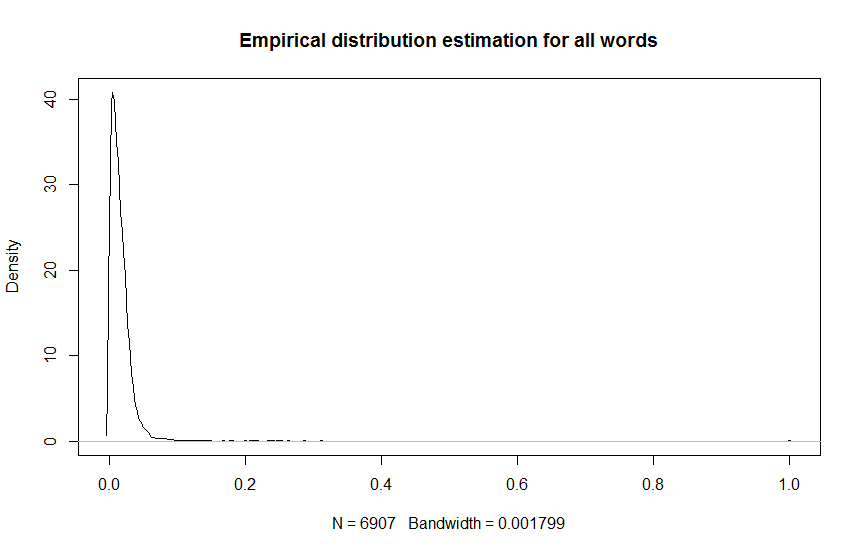
\includegraphics[scale=0.5]{./Figures/all.png}
\label{all}
\end{figure}

\begin{figure}[! ht]
\centering
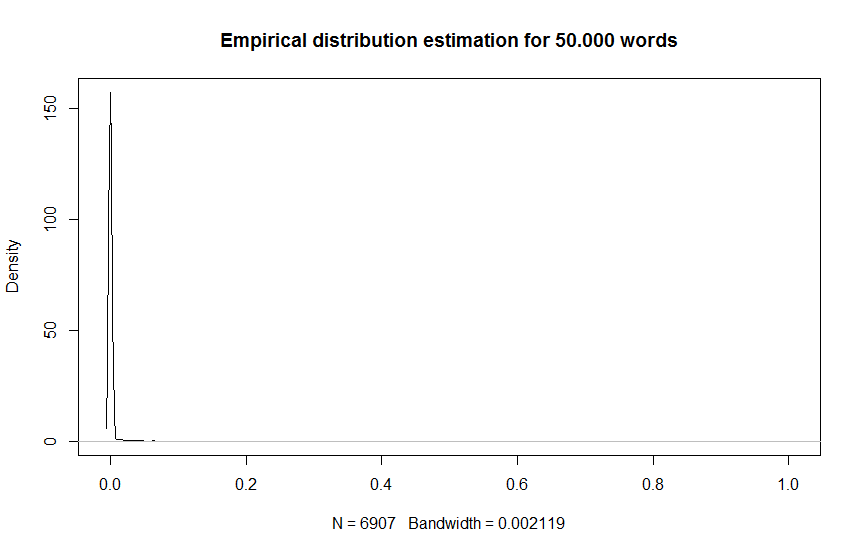
\includegraphics[scale=0.5]{./Figures/50.png}
\label{50}
\end{figure}

\begin{figure}[! ht]
\centering
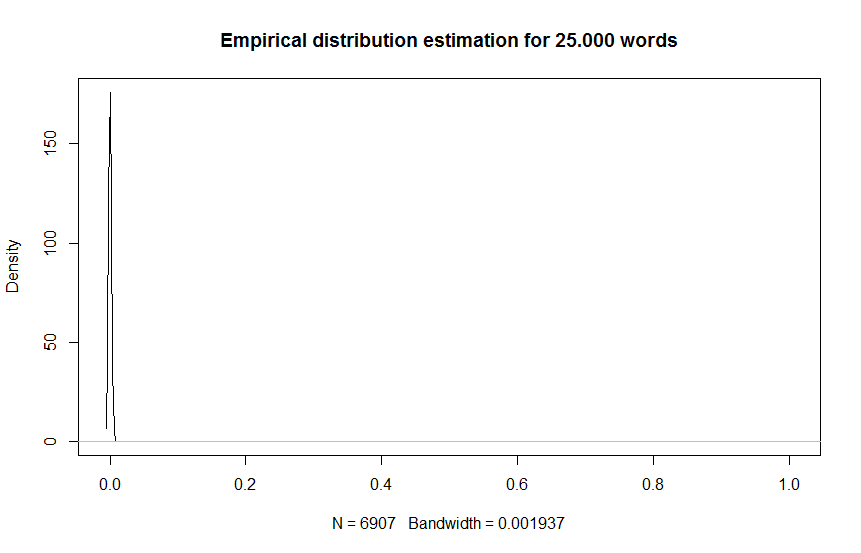
\includegraphics[scale=0.5]{./Figures/25.png}
\label{25}
\end{figure}

\begin{figure}[! ht]
\centering
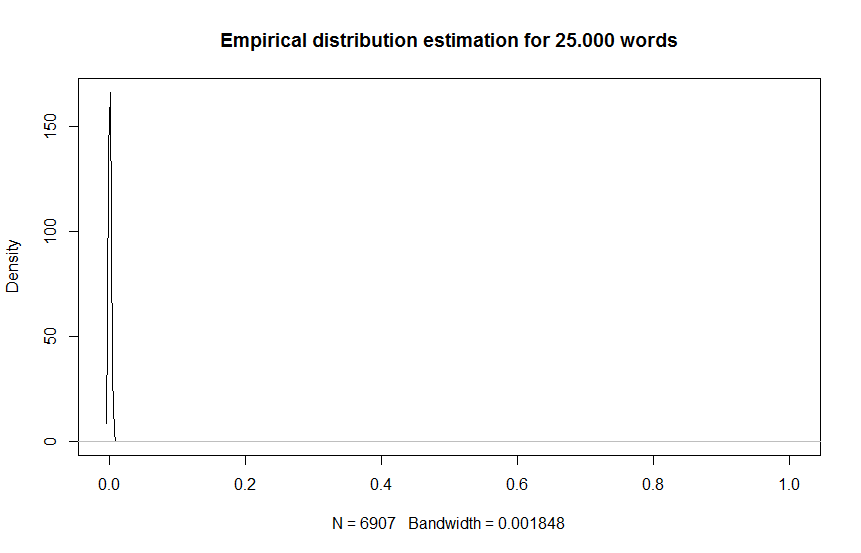
\includegraphics[scale=0.5]{./Figures/10.png}
\label{10}
\end{figure}

\pagebreak

These distributions are an Inverse Gaussian distributions. We can see that as the vocabulary decreases, the shape factor $\lambda$ decreases, giving the distribution a more and more narrow appearance (as opposed to increasing it, which makes the distribution resemble a Normal distribution).


\section{The underpinnings of Log-Entropy}
\subsection{Why is there a ‘+1’ in the logarithm function ?}
It is simply because the logarithm function is defined on the domain of the strictly positive real: it is possible for $tf_{ij}$ to be equal to 0 simply because of it's definition: it is possible the $i^{th}$ document does not contain the $j^{th}$ therm. Hence, the '+1' allows us to shift the domain of $tf_{ij}$ from $[0,\; \vert\vert document_i \vert\vert ]$ to $[1,\; \vert\vert document_i \vert\vert +1 ]$ on which the logarithm function is entirely defined.
\subsection{What is the point to apply the logarithm function to the term frequency instead of plugging it directly in the formula ?}
This allows us to diminish the relative importance of the high frequency words versus the middle ones. Indeed, the logarithm function is defined so that, compared with the linear function suggested, it keeps the middle frequencies importance while really lowering the high frequencies. This effect allows us to take into account the fact that some words tends to appear in every document while not being decisive for de description of the document (words such as "the", "a", "b", etc.). Moreover, some other words only appear a few times in the document in question while being really important for the definition/description of it; the importance of theses words is better taken into account by the logarithm function than by the linear one.
\subsection{Could explain intuitively the mechanics of the global weight ? And why is there a division by log n? (Hint: What does the entropy of a distribution represents?)}
First, let us remark that the global weight can easily be written as: \begin{equation}
g_{ij} = 1 - \frac{-\Sigma_i\; p_{ij}\cdot \log p_{ij}}{\log n}
\end{equation}
With this particular notation, the resemblance with formula of the entropy for the distribution $p_{ij}$ is quite hard to miss ($\Sigma_i\; p_{ij}\cdot \log p_{ij}$). This entropy measures the uncertainty of the location of $j^{th}$ in the $i^{th}$ document. Now we focus on the division by the $\log n$ which is simple too: the maximum value of this entropy is actually $\log n$ meaning that we project the domain of the entropy of the distribution onto a domain bounded by 0 and 1. Then, we inverse the sense of the domain by the operation of subtraction: this allows us to define a greater weight for the terms that more certain (with less uncertainty) to be present in the document. Moreover, this also allows us to give a greater weight to the terms that a specific to this document by lowering the one of the terms that are more likely to appear in each document.
\end{document}  